\documentclass[twoside]{article}

% Packages required by doxygen
\usepackage{fixltx2e}
\usepackage{calc}
\usepackage{doxygen}
\usepackage{graphicx}
\usepackage[utf8]{inputenc}
\usepackage{makeidx}
\usepackage{multicol}
\usepackage{multirow}
\PassOptionsToPackage{warn}{textcomp}
\usepackage{textcomp}
\usepackage[nointegrals]{wasysym}
\usepackage[table]{xcolor}

% Font selection
\usepackage[T1]{fontenc}
\usepackage{mathptmx}
\usepackage[scaled=.90]{helvet}
\usepackage{courier}
\usepackage{amssymb}
\usepackage{sectsty}
\renewcommand{\familydefault}{\sfdefault}
\allsectionsfont{%
  \fontseries{bc}\selectfont%
  \color{darkgray}%
}
\renewcommand{\DoxyLabelFont}{%
  \fontseries{bc}\selectfont%
  \color{darkgray}%
}
\newcommand{\+}{\discretionary{\mbox{\scriptsize$\hookleftarrow$}}{}{}}

% Page & text layout
\usepackage[screen]{geometry}
\tolerance=750
\hfuzz=15pt
\hbadness=750
\setlength{\emergencystretch}{15pt}
\setlength{\parindent}{0cm}
\setlength{\parskip}{0.2cm}
\makeatletter
\renewcommand{\paragraph}{%
  \@startsection{paragraph}{4}{0ex}{-1.0ex}{1.0ex}{%
    \normalfont\normalsize\bfseries\SS@parafont%
  }%
}
\renewcommand{\subparagraph}{%
  \@startsection{subparagraph}{5}{0ex}{-1.0ex}{1.0ex}{%
    \normalfont\normalsize\bfseries\SS@subparafont%
  }%
}
\makeatother

% Headers & footers
\usepackage{fancyhdr}
\pagestyle{fancyplain}
\fancyhead[LE]{\fancyplain{}{\bfseries\thepage}}
\fancyhead[CE]{\fancyplain{}{}}
\fancyhead[RE]{\fancyplain{}{\bfseries\leftmark}}
\fancyhead[LO]{\fancyplain{}{\bfseries\rightmark}}
\fancyhead[CO]{\fancyplain{}{}}
\fancyhead[RO]{\fancyplain{}{\bfseries\thepage}}
\fancyfoot[LE]{\fancyplain{}{}}
\fancyfoot[CE]{\fancyplain{}{}}
\fancyfoot[RE]{\fancyplain{}{\bfseries\scriptsize Generated on Wed Nov 1 2017 00\+:15\+:27 by Doxygen }}
\fancyfoot[LO]{\fancyplain{}{\bfseries\scriptsize Generated on Wed Nov 1 2017 00\+:15\+:27 by Doxygen }}
\fancyfoot[CO]{\fancyplain{}{}}
\fancyfoot[RO]{\fancyplain{}{}}
\renewcommand{\footrulewidth}{0.4pt}
\renewcommand{\sectionmark}[1]{%
  \markright{\thesection\ #1}%
}

% Indices & bibliography
\usepackage{natbib}
\usepackage[titles]{tocloft}
\setcounter{tocdepth}{3}
\setcounter{secnumdepth}{5}
\makeindex

% Packages requested by user
\usepackage{titlesec}

% Hyperlinks (required, but should be loaded last)
\usepackage{ifpdf}
\ifpdf
  \usepackage[pdftex,pagebackref=true]{hyperref}
\else
  \usepackage[ps2pdf,pagebackref=true]{hyperref}
\fi
\hypersetup{%
  colorlinks=true,%
  linkcolor=blue,%
  citecolor=blue,%
  unicode%
}

% Custom commands
\newcommand{\clearemptydoublepage}{%
  \newpage{\pagestyle{empty}\cleardoublepage}%
}


\newcommand{\sectionbreak}{\clearpage}

\begin{document}

% Titlepage & ToC
\hypersetup{pageanchor=false,
             bookmarks=true,
             bookmarksnumbered=true,
             pdfencoding=unicode
            }
\pagenumbering{roman}
\begin{titlepage}
\vspace*{7cm}
\begin{center}%
{\Large Reference Manual}\\
\vspace*{1cm}
{\large Generated by Doxygen 1.8.8}\\
\vspace*{0.5cm}
{\small Wed Nov 1 2017 00:15:27}\\
\end{center}
\end{titlepage}
\tableofcontents
\pagenumbering{arabic}
\hypersetup{pageanchor=true}

%--- Begin generated contents ---
\section{count\+Rows}
\label{countRows}
\hypertarget{countRows}{}
Read the first string in file f return it. 
\section{read\+Data}
\label{readData}
\hypertarget{readData}{}
Read the first string in file f return it.


\begin{DoxyParams}{Parameters}
{\em f} & filename \\
\hline
{\em aqi\mbox{[}$\,$\mbox{]}} & is an array to put data in /param n number amount of elements in the array \\
\hline
\end{DoxyParams}
\begin{DoxyReturn}{Returns}
void 
\end{DoxyReturn}

\section{Class Index}
\subsection{Class List}
Here are the classes, structs, unions and interfaces with brief descriptions\+:\begin{DoxyCompactList}
\item\contentsline{section}{\hyperlink{structENTRY}{E\+N\+T\+R\+Y} }{\pageref{structENTRY}}{}
\end{DoxyCompactList}

\section{File Index}
\subsection{File List}
Here is a list of all files with brief descriptions\+:\begin{DoxyCompactList}
\item\contentsline{section}{\hyperlink{BuildListDirectly_8cpp}{Build\+List\+Directly.\+cpp} }{\pageref{BuildListDirectly_8cpp}}{}
\item\contentsline{section}{\hyperlink{destroyList_8cpp}{destroy\+List.\+cpp} }{\pageref{destroyList_8cpp}}{}
\item\contentsline{section}{\hyperlink{displayList_8cpp}{display\+List.\+cpp} }{\pageref{displayList_8cpp}}{}
\item\contentsline{section}{\hyperlink{Insert_8cpp}{Insert.\+cpp} }{\pageref{Insert_8cpp}}{}
\item\contentsline{section}{\hyperlink{InsertInOrder_8cpp}{Insert\+In\+Order.\+cpp} }{\pageref{InsertInOrder_8cpp}}{}
\item\contentsline{section}{\hyperlink{lab2_8h}{lab2.\+h} }{\pageref{lab2_8h}}{}
\item\contentsline{section}{\hyperlink{loadList_8cpp}{load\+List.\+cpp} }{\pageref{loadList_8cpp}}{}
\item\contentsline{section}{\hyperlink{loadList2_8cpp}{load\+List2.\+cpp} }{\pageref{loadList2_8cpp}}{}
\item\contentsline{section}{\hyperlink{loadList3_8cpp}{load\+List3.\+cpp} }{\pageref{loadList3_8cpp}}{}
\item\contentsline{section}{\hyperlink{main_8cpp}{main.\+cpp} }{\pageref{main_8cpp}}{}
\end{DoxyCompactList}

\section{Class Documentation}
\hypertarget{structAQIData}{\subsection{A\+Q\+I\+Data Struct Reference}
\label{structAQIData}\index{A\+Q\+I\+Data@{A\+Q\+I\+Data}}
}


{\ttfamily \#include $<$lab.\+h$>$}

\subsubsection*{Public Attributes}
\begin{DoxyCompactItemize}
\item 
std\+::string \hyperlink{structAQIData_af9ac1abc791a7df144f3dba5c53c0f1a}{county}
\item 
std\+::string \hyperlink{structAQIData_a5077140b5e97ceba8b82a776647fb667}{A\+Q\+I}
\end{DoxyCompactItemize}


\subsubsection{Member Data Documentation}
\hypertarget{structAQIData_a5077140b5e97ceba8b82a776647fb667}{\index{A\+Q\+I\+Data@{A\+Q\+I\+Data}!A\+Q\+I@{A\+Q\+I}}
\index{A\+Q\+I@{A\+Q\+I}!A\+Q\+I\+Data@{A\+Q\+I\+Data}}
\paragraph[{A\+Q\+I}]{\setlength{\rightskip}{0pt plus 5cm}std\+::string A\+Q\+I\+Data\+::\+A\+Q\+I}}\label{structAQIData_a5077140b5e97ceba8b82a776647fb667}
\hypertarget{structAQIData_af9ac1abc791a7df144f3dba5c53c0f1a}{\index{A\+Q\+I\+Data@{A\+Q\+I\+Data}!county@{county}}
\index{county@{county}!A\+Q\+I\+Data@{A\+Q\+I\+Data}}
\paragraph[{county}]{\setlength{\rightskip}{0pt plus 5cm}std\+::string A\+Q\+I\+Data\+::county}}\label{structAQIData_af9ac1abc791a7df144f3dba5c53c0f1a}


The documentation for this struct was generated from the following file\+:\begin{DoxyCompactItemize}
\item 
\hyperlink{lab_8h}{lab.\+h}\end{DoxyCompactItemize}

\hypertarget{classMERGESORT}{\subsection{M\+E\+R\+G\+E\+S\+O\+R\+T$<$ S\+O\+M\+E\+T\+Y\+P\+E $>$ Class Template Reference}
\label{classMERGESORT}\index{M\+E\+R\+G\+E\+S\+O\+R\+T$<$ S\+O\+M\+E\+T\+Y\+P\+E $>$@{M\+E\+R\+G\+E\+S\+O\+R\+T$<$ S\+O\+M\+E\+T\+Y\+P\+E $>$}}
}


{\ttfamily \#include $<$lab.\+h$>$}

\subsubsection*{Public Member Functions}
\begin{DoxyCompactItemize}
\item 
\hyperlink{classMERGESORT_ae2b246469efd38d5bed5da71e38cb3ea}{M\+E\+R\+G\+E\+S\+O\+R\+T} (int n)
\item 
\hyperlink{classMERGESORT_a28eb2ff8548afa8ceb90ec38f567dbb8}{$\sim$\+M\+E\+R\+G\+E\+S\+O\+R\+T} ()
\item 
void \hyperlink{classMERGESORT_a8af2add54cd2f739b68dca4750704c6c}{Sort} (S\+O\+M\+E\+T\+Y\+P\+E a\mbox{[}$\,$\mbox{]}, int n)
\end{DoxyCompactItemize}


\subsubsection{Constructor \& Destructor Documentation}
\hypertarget{classMERGESORT_ae2b246469efd38d5bed5da71e38cb3ea}{\index{M\+E\+R\+G\+E\+S\+O\+R\+T@{M\+E\+R\+G\+E\+S\+O\+R\+T}!M\+E\+R\+G\+E\+S\+O\+R\+T@{M\+E\+R\+G\+E\+S\+O\+R\+T}}
\index{M\+E\+R\+G\+E\+S\+O\+R\+T@{M\+E\+R\+G\+E\+S\+O\+R\+T}!M\+E\+R\+G\+E\+S\+O\+R\+T@{M\+E\+R\+G\+E\+S\+O\+R\+T}}
\paragraph[{M\+E\+R\+G\+E\+S\+O\+R\+T}]{\setlength{\rightskip}{0pt plus 5cm}template$<$class S\+O\+M\+E\+T\+Y\+P\+E$>$ {\bf M\+E\+R\+G\+E\+S\+O\+R\+T}$<$ S\+O\+M\+E\+T\+Y\+P\+E $>$\+::{\bf M\+E\+R\+G\+E\+S\+O\+R\+T} (
\begin{DoxyParamCaption}
\item[{int}]{n}
\end{DoxyParamCaption}
)\hspace{0.3cm}{\ttfamily [inline]}}}\label{classMERGESORT_ae2b246469efd38d5bed5da71e38cb3ea}

\begin{DoxyCode}
31 \{ work = \textcolor{keyword}{new} SOMETYPE[n]; \}
\end{DoxyCode}
\hypertarget{classMERGESORT_a28eb2ff8548afa8ceb90ec38f567dbb8}{\index{M\+E\+R\+G\+E\+S\+O\+R\+T@{M\+E\+R\+G\+E\+S\+O\+R\+T}!````~M\+E\+R\+G\+E\+S\+O\+R\+T@{$\sim$\+M\+E\+R\+G\+E\+S\+O\+R\+T}}
\index{````~M\+E\+R\+G\+E\+S\+O\+R\+T@{$\sim$\+M\+E\+R\+G\+E\+S\+O\+R\+T}!M\+E\+R\+G\+E\+S\+O\+R\+T@{M\+E\+R\+G\+E\+S\+O\+R\+T}}
\paragraph[{$\sim$\+M\+E\+R\+G\+E\+S\+O\+R\+T}]{\setlength{\rightskip}{0pt plus 5cm}template$<$class S\+O\+M\+E\+T\+Y\+P\+E$>$ {\bf M\+E\+R\+G\+E\+S\+O\+R\+T}$<$ S\+O\+M\+E\+T\+Y\+P\+E $>$\+::$\sim${\bf M\+E\+R\+G\+E\+S\+O\+R\+T} (
\begin{DoxyParamCaption}
{}
\end{DoxyParamCaption}
)\hspace{0.3cm}{\ttfamily [inline]}}}\label{classMERGESORT_a28eb2ff8548afa8ceb90ec38f567dbb8}

\begin{DoxyCode}
33 \{ \textcolor{keyword}{delete} [] work; \}
\end{DoxyCode}


\subsubsection{Member Function Documentation}
\hypertarget{classMERGESORT_a8af2add54cd2f739b68dca4750704c6c}{\index{M\+E\+R\+G\+E\+S\+O\+R\+T@{M\+E\+R\+G\+E\+S\+O\+R\+T}!Sort@{Sort}}
\index{Sort@{Sort}!M\+E\+R\+G\+E\+S\+O\+R\+T@{M\+E\+R\+G\+E\+S\+O\+R\+T}}
\paragraph[{Sort}]{\setlength{\rightskip}{0pt plus 5cm}template$<$class S\+O\+M\+E\+T\+Y\+P\+E $>$ void {\bf M\+E\+R\+G\+E\+S\+O\+R\+T}$<$ S\+O\+M\+E\+T\+Y\+P\+E $>$\+::Sort (
\begin{DoxyParamCaption}
\item[{S\+O\+M\+E\+T\+Y\+P\+E}]{a\mbox{[}$\,$\mbox{]}, }
\item[{int}]{n}
\end{DoxyParamCaption}
)}}\label{classMERGESORT_a8af2add54cd2f739b68dca4750704c6c}

\begin{DoxyCode}
61 \{
62     \{
63     \textcolor{keywordtype}{int} n1, n2;
64     SOMETYPE *a2;
65     \textcolor{keywordflow}{if} (n <= 2) \{ \textcolor{comment}{// Base case:}
66         \textcolor{keywordflow}{if} (n == 2 && a[1] < a[0])
67             Swap(a[0], a[1]);
68     \}
69     \textcolor{keywordflow}{else} \{ \textcolor{comment}{// Recursive case:}
70         n1 = n/2; n2 = n - n1;
71         a2 = &a[n1]; \textcolor{comment}{// a2 points to the second half of the}
72         \textcolor{comment}{// array.}
73         \hyperlink{classMERGESORT_a8af2add54cd2f739b68dca4750704c6c}{Sort}(a, n1);
74         \hyperlink{classMERGESORT_a8af2add54cd2f739b68dca4750704c6c}{Sort}(a2, n2);
75         Merge(a, n1, a2, n2);
76     \}
77 \}
78 \}
\end{DoxyCode}


The documentation for this class was generated from the following files\+:\begin{DoxyCompactItemize}
\item 
\hyperlink{lab_8h}{lab.\+h}\item 
\hyperlink{lab_8hpp}{lab.\+hpp}\end{DoxyCompactItemize}

\hypertarget{classQUICKSORT}{\subsection{Q\+U\+I\+C\+K\+S\+O\+R\+T$<$ S\+O\+M\+E\+T\+Y\+P\+E $>$ Class Template Reference}
\label{classQUICKSORT}\index{Q\+U\+I\+C\+K\+S\+O\+R\+T$<$ S\+O\+M\+E\+T\+Y\+P\+E $>$@{Q\+U\+I\+C\+K\+S\+O\+R\+T$<$ S\+O\+M\+E\+T\+Y\+P\+E $>$}}
}


{\ttfamily \#include $<$lab.\+h$>$}

\subsubsection*{Public Member Functions}
\begin{DoxyCompactItemize}
\item 
void \hyperlink{classQUICKSORT_a64941ba9af48331a00ef8d8de38c54b6}{Sort} (S\+O\+M\+E\+T\+Y\+P\+E a\mbox{[}$\,$\mbox{]}, int n)
\end{DoxyCompactItemize}


\subsubsection{Member Function Documentation}
\hypertarget{classQUICKSORT_a64941ba9af48331a00ef8d8de38c54b6}{\index{Q\+U\+I\+C\+K\+S\+O\+R\+T@{Q\+U\+I\+C\+K\+S\+O\+R\+T}!Sort@{Sort}}
\index{Sort@{Sort}!Q\+U\+I\+C\+K\+S\+O\+R\+T@{Q\+U\+I\+C\+K\+S\+O\+R\+T}}
\paragraph[{Sort}]{\setlength{\rightskip}{0pt plus 5cm}template$<$class S\+O\+M\+E\+T\+Y\+P\+E$>$ void {\bf Q\+U\+I\+C\+K\+S\+O\+R\+T}$<$ S\+O\+M\+E\+T\+Y\+P\+E $>$\+::Sort (
\begin{DoxyParamCaption}
\item[{S\+O\+M\+E\+T\+Y\+P\+E}]{a\mbox{[}$\,$\mbox{]}, }
\item[{int}]{n}
\end{DoxyParamCaption}
)}}\label{classQUICKSORT_a64941ba9af48331a00ef8d8de38c54b6}


The documentation for this class was generated from the following files\+:\begin{DoxyCompactItemize}
\item 
\hyperlink{lab_8h}{lab.\+h}\item 
\hyperlink{lab_8hpp}{lab.\+hpp}\end{DoxyCompactItemize}

\section{File Documentation}
\hypertarget{countRows_8cpp}{\subsection{count\+Rows.\+cpp File Reference}
\label{countRows_8cpp}\index{count\+Rows.\+cpp@{count\+Rows.\+cpp}}
}
{\ttfamily \#include \char`\"{}lab.\+h\char`\"{}}\\*
Include dependency graph for count\+Rows.\+cpp\+:\nopagebreak
\begin{figure}[H]
\begin{center}
\leavevmode
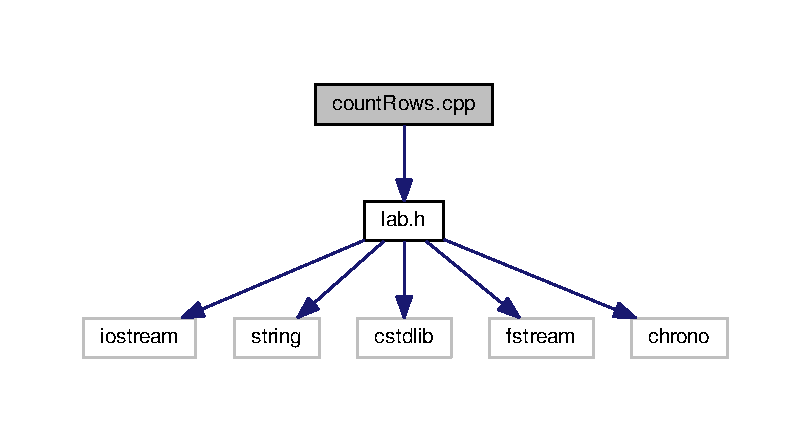
\includegraphics[width=350pt]{countRows_8cpp__incl}
\end{center}
\end{figure}
\subsubsection*{Functions}
\begin{DoxyCompactItemize}
\item 
int \hyperlink{countRows_8cpp_a15de8e3dda2c911202abcc072d075935}{count\+Rows} (std\+::string f)
\end{DoxyCompactItemize}


\subsubsection{Function Documentation}
\hypertarget{countRows_8cpp_a15de8e3dda2c911202abcc072d075935}{\index{count\+Rows.\+cpp@{count\+Rows.\+cpp}!count\+Rows@{count\+Rows}}
\index{count\+Rows@{count\+Rows}!count\+Rows.\+cpp@{count\+Rows.\+cpp}}
\paragraph[{count\+Rows}]{\setlength{\rightskip}{0pt plus 5cm}int count\+Rows (
\begin{DoxyParamCaption}
\item[{std\+::string}]{f}
\end{DoxyParamCaption}
)}}\label{countRows_8cpp_a15de8e3dda2c911202abcc072d075935}

\begin{DoxyCode}
4 \{   
5     std::ifstream ifs(f.c\_str());
6     \textcolor{keywordtype}{int} n = 0;
7     std::string s;
8     \textcolor{keywordflow}{while}(getline(ifs,s)) n++;
9     ifs.close();
10     \textcolor{keywordflow}{return} n;
11 \}
\end{DoxyCode}

\hypertarget{lab_8h}{\subsection{lab.\+h File Reference}
\label{lab_8h}\index{lab.\+h@{lab.\+h}}
}
{\ttfamily \#include \char`\"{}config.\+h\char`\"{}}\\*
{\ttfamily \#include $<$F\+L/\+Fl\+\_\+\+Cairo\+\_\+\+Window.\+H$>$}\\*
{\ttfamily \#include $<$F\+L/\+Fl\+\_\+\+Input.\+H$>$}\\*
{\ttfamily \#include $<$F\+L/\+Fl\+\_\+\+Button.\+H$>$}\\*
{\ttfamily \#include $<$F\+L/fl\+\_\+ask.\+H$>$}\\*
{\ttfamily \#include $<$iostream$>$}\\*
{\ttfamily \#include $<$F\+L/\+Fl\+\_\+\+Output.\+H$>$}\\*
{\ttfamily \#include $<$sstream$>$}\\*
{\ttfamily \#include $<$iomanip$>$}\\*
{\ttfamily \#include $<$F\+L/\+Fl\+\_\+\+Text\+\_\+\+Display.\+H$>$}\\*
{\ttfamily \#include $<$F\+L/\+Fl\+\_\+\+Text\+\_\+\+Buffer.\+H$>$}\\*
Include dependency graph for lab.\+h\+:\nopagebreak
\begin{figure}[H]
\begin{center}
\leavevmode
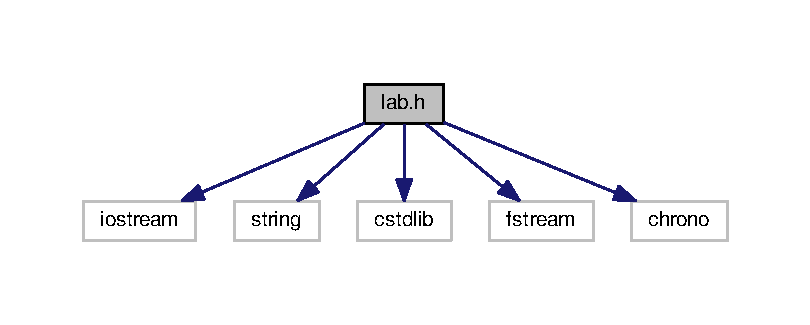
\includegraphics[width=350pt]{lab_8h__incl}
\end{center}
\end{figure}
This graph shows which files directly or indirectly include this file\+:\nopagebreak
\begin{figure}[H]
\begin{center}
\leavevmode
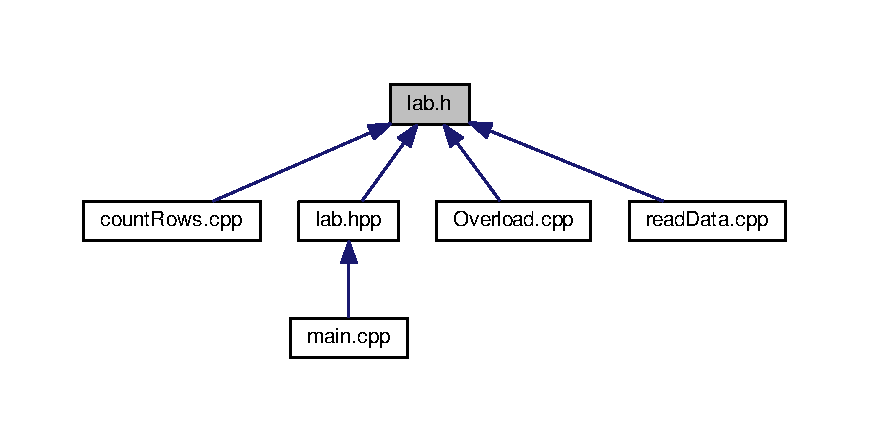
\includegraphics[width=350pt]{lab_8h__dep__incl}
\end{center}
\end{figure}
\subsubsection*{Functions}
\begin{DoxyCompactItemize}
\item 
void \hyperlink{lab_8h_a547f84331a8c529348e1130ca169c69c}{order\+\_\+cb} (void $\ast$, void $\ast$)
\item 
void \hyperlink{lab_8h_abb6fd11336b6e04e134b70abc225a8f6}{cook\+\_\+cb} (void $\ast$)
\item 
void \hyperlink{lab_8h_a13ed8751dfa95731ad8930762493b16b}{timer} (void $\ast$)
\end{DoxyCompactItemize}
\subsubsection*{Variables}
\begin{DoxyCompactItemize}
\item 
Fl\+\_\+\+Input $\ast$ \hyperlink{lab_8h_abf805c82a90897837d1c26ef915f1cd6}{pizza}
\item 
Fl\+\_\+\+Output $\ast$ \hyperlink{lab_8h_a05c7f6e86cca5f4d0ebf44d1f5042c37}{watch}
\item 
Fl\+\_\+\+Text\+\_\+\+Buffer $\ast$ \hyperlink{lab_8h_aea2b8efadc87a819fe57c311d668e504}{buff}
\item 
Fl\+\_\+\+Text\+\_\+\+Display $\ast$ \hyperlink{lab_8h_a23f917547a833922fd6bc8797cc04ee1}{order\+Q}
\end{DoxyCompactItemize}


\subsubsection{Function Documentation}
\hypertarget{lab_8h_abb6fd11336b6e04e134b70abc225a8f6}{\index{lab.\+h@{lab.\+h}!cook\+\_\+cb@{cook\+\_\+cb}}
\index{cook\+\_\+cb@{cook\+\_\+cb}!lab.\+h@{lab.\+h}}
\paragraph[{cook\+\_\+cb}]{\setlength{\rightskip}{0pt plus 5cm}void cook\+\_\+cb (
\begin{DoxyParamCaption}
\item[{void $\ast$}]{}
\end{DoxyParamCaption}
)}}\label{lab_8h_abb6fd11336b6e04e134b70abc225a8f6}

\begin{DoxyCode}
3 \{
4     \textcolor{comment}{//buff->text(pizza->value());}
5     
6     \textcolor{comment}{// temp solution, when it's cooked, put it}
7     \textcolor{comment}{// in the LLQueue; then here }
8     \textcolor{comment}{// use your new function that displays}
9     \textcolor{comment}{// what is in Q to create a string (with newlines)}
10     \textcolor{comment}{// in it, return it here and siplay that in the buffer}
11     
12 \}
\end{DoxyCode}
\hypertarget{lab_8h_a547f84331a8c529348e1130ca169c69c}{\index{lab.\+h@{lab.\+h}!order\+\_\+cb@{order\+\_\+cb}}
\index{order\+\_\+cb@{order\+\_\+cb}!lab.\+h@{lab.\+h}}
\paragraph[{order\+\_\+cb}]{\setlength{\rightskip}{0pt plus 5cm}void order\+\_\+cb (
\begin{DoxyParamCaption}
\item[{void $\ast$}]{, }
\item[{void $\ast$}]{}
\end{DoxyParamCaption}
)}}\label{lab_8h_a547f84331a8c529348e1130ca169c69c}

\begin{DoxyCode}
3 \{
4     fl\_alert(\hyperlink{lab_8h_abf805c82a90897837d1c26ef915f1cd6}{pizza}->value());
5     \textcolor{comment}{// cook it}
6     Fl::add\_timeout(5,\hyperlink{cook__cb_8cpp_abb6fd11336b6e04e134b70abc225a8f6}{cook\_cb});
7 \}
\end{DoxyCode}
\hypertarget{lab_8h_a13ed8751dfa95731ad8930762493b16b}{\index{lab.\+h@{lab.\+h}!timer@{timer}}
\index{timer@{timer}!lab.\+h@{lab.\+h}}
\paragraph[{timer}]{\setlength{\rightskip}{0pt plus 5cm}void timer (
\begin{DoxyParamCaption}
\item[{void $\ast$}]{}
\end{DoxyParamCaption}
)}}\label{lab_8h_a13ed8751dfa95731ad8930762493b16b}

\begin{DoxyCode}
3 \{
4     \textcolor{comment}{//std::cout << "1 sec" << std::endl;}
5     \textcolor{keyword}{static} \textcolor{keywordtype}{int} s= 0; \textcolor{keyword}{static} \textcolor{keywordtype}{int} m = 0;
6     std::ostringstream oss; \textcolor{comment}{// don't discard the memory. }
7                                               \textcolor{comment}{// keep it so we can update t to the window}
8     s++;    \textcolor{keywordflow}{if}(s == 59) \{s = 0; m++; \}
9     oss << std::setfill(\textcolor{charliteral}{'0'});
10     oss << std::setw(2) << m << \textcolor{stringliteral}{":"} << std::setw(2) << s;
11     \textcolor{comment}{//oss << s;}
12     \hyperlink{lab_8h_a05c7f6e86cca5f4d0ebf44d1f5042c37}{watch}->value(oss.str().c\_str());
13     
14     \textcolor{comment}{// Here we could check if the Q's have pizza and drivers}
15     \textcolor{comment}{// ready for delivery every 10 seconds so we can see order}
16     \textcolor{comment}{// in Q     if (s % 10 == 0)}
17     \textcolor{keyword}{static} std::string str;
18     std::string pizzas[] = \{\textcolor{stringliteral}{"veggie"},\textcolor{stringliteral}{"pepperoni"},\textcolor{stringliteral}{"sausage"},\textcolor{stringliteral}{"hawaiian"}\};
19     \textcolor{keywordflow}{if}(s % 10 == 0)
20     \{
21         str += pizzas[s%4] += \textcolor{stringliteral}{"\(\backslash\)n"};
22         \hyperlink{lab_8h_aea2b8efadc87a819fe57c311d668e504}{buff}->text(str.c\_str());
23     \}
24     
25     Fl::repeat\_timeout(1,\hyperlink{timer_8cpp_a13ed8751dfa95731ad8930762493b16b}{timer});
26 \}
\end{DoxyCode}


\subsubsection{Variable Documentation}
\hypertarget{lab_8h_aea2b8efadc87a819fe57c311d668e504}{\index{lab.\+h@{lab.\+h}!buff@{buff}}
\index{buff@{buff}!lab.\+h@{lab.\+h}}
\paragraph[{buff}]{\setlength{\rightskip}{0pt plus 5cm}Fl\+\_\+\+Text\+\_\+\+Buffer$\ast$ buff}}\label{lab_8h_aea2b8efadc87a819fe57c311d668e504}
\hypertarget{lab_8h_a23f917547a833922fd6bc8797cc04ee1}{\index{lab.\+h@{lab.\+h}!order\+Q@{order\+Q}}
\index{order\+Q@{order\+Q}!lab.\+h@{lab.\+h}}
\paragraph[{order\+Q}]{\setlength{\rightskip}{0pt plus 5cm}Fl\+\_\+\+Text\+\_\+\+Display$\ast$ order\+Q}}\label{lab_8h_a23f917547a833922fd6bc8797cc04ee1}
\hypertarget{lab_8h_abf805c82a90897837d1c26ef915f1cd6}{\index{lab.\+h@{lab.\+h}!pizza@{pizza}}
\index{pizza@{pizza}!lab.\+h@{lab.\+h}}
\paragraph[{pizza}]{\setlength{\rightskip}{0pt plus 5cm}Fl\+\_\+\+Input$\ast$ pizza}}\label{lab_8h_abf805c82a90897837d1c26ef915f1cd6}
\hypertarget{lab_8h_a05c7f6e86cca5f4d0ebf44d1f5042c37}{\index{lab.\+h@{lab.\+h}!watch@{watch}}
\index{watch@{watch}!lab.\+h@{lab.\+h}}
\paragraph[{watch}]{\setlength{\rightskip}{0pt plus 5cm}Fl\+\_\+\+Output$\ast$ watch}}\label{lab_8h_a05c7f6e86cca5f4d0ebf44d1f5042c37}

\hypertarget{lab_8hpp}{\subsection{lab.\+hpp File Reference}
\label{lab_8hpp}\index{lab.\+hpp@{lab.\+hpp}}
}
{\ttfamily \#include \char`\"{}lab.\+h\char`\"{}}\\*
Include dependency graph for lab.\+hpp\+:
\nopagebreak
\begin{figure}[H]
\begin{center}
\leavevmode
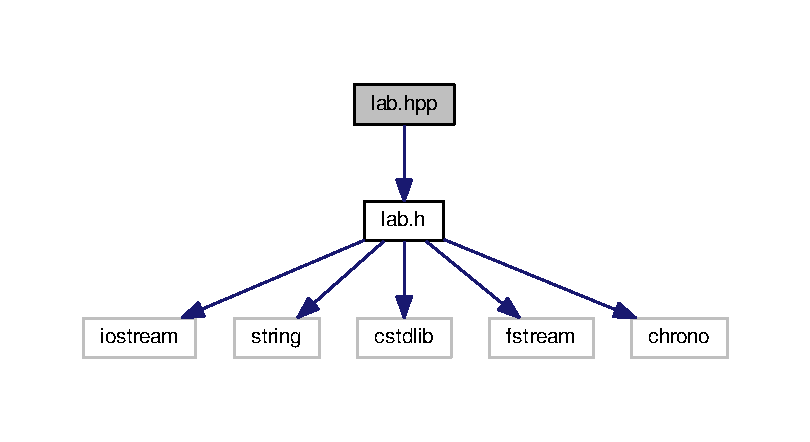
\includegraphics[width=350pt]{lab_8hpp__incl}
\end{center}
\end{figure}
This graph shows which files directly or indirectly include this file\+:
\nopagebreak
\begin{figure}[H]
\begin{center}
\leavevmode
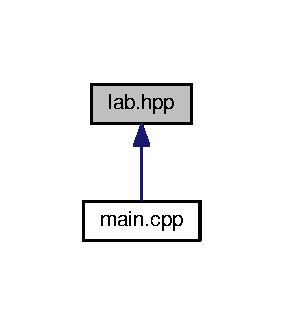
\includegraphics[width=136pt]{lab_8hpp__dep__incl}
\end{center}
\end{figure}
\subsubsection*{Functions}
\begin{DoxyCompactItemize}
\item 
{\footnotesize template$<$class S\+O\+M\+E\+T\+Y\+P\+E $>$ }\\void \hyperlink{lab_8hpp_a1ec382402a95cebbc33fe53598278275}{Swap} (S\+O\+M\+E\+T\+Y\+P\+E \&a, S\+O\+M\+E\+T\+Y\+P\+E \&b)
\item 
{\footnotesize template$<$class S\+O\+M\+E\+T\+Y\+P\+E $>$ }\\void \hyperlink{lab_8hpp_ac885c8287654c56c998ed7a7c9f334eb}{Selection\+Sort} (S\+O\+M\+E\+T\+Y\+P\+E a\mbox{[}$\,$\mbox{]}, int n)
\item 
{\footnotesize template$<$class S\+O\+M\+E\+T\+Y\+P\+E $>$ }\\void \hyperlink{lab_8hpp_a03ccf968e02545e2d24fe6427e5b9f16}{Insertion\+Sort} (S\+O\+M\+E\+T\+Y\+P\+E a\mbox{[}$\,$\mbox{]}, int n)
\item 
{\footnotesize template$<$class S\+O\+M\+E\+T\+Y\+P\+E $>$ }\\void \hyperlink{lab_8hpp_abed8a965e2fc3713a88fee0e7f11ad1e}{Bubble\+Sort} (S\+O\+M\+E\+T\+Y\+P\+E a\mbox{[}$\,$\mbox{]}, int n)
\end{DoxyCompactItemize}


\subsubsection{Function Documentation}
\hypertarget{lab_8hpp_abed8a965e2fc3713a88fee0e7f11ad1e}{\index{lab.\+hpp@{lab.\+hpp}!Bubble\+Sort@{Bubble\+Sort}}
\index{Bubble\+Sort@{Bubble\+Sort}!lab.\+hpp@{lab.\+hpp}}
\paragraph[{Bubble\+Sort}]{\setlength{\rightskip}{0pt plus 5cm}template$<$class S\+O\+M\+E\+T\+Y\+P\+E $>$ void Bubble\+Sort (
\begin{DoxyParamCaption}
\item[{S\+O\+M\+E\+T\+Y\+P\+E}]{a\mbox{[}$\,$\mbox{]}, }
\item[{int}]{n}
\end{DoxyParamCaption}
)}}\label{lab_8hpp_abed8a965e2fc3713a88fee0e7f11ad1e}

\begin{DoxyCode}
42 \{
43     \textcolor{keywordtype}{int} i, disorder = n;
44     \textcolor{keywordflow}{while}(disorder)
45     \{
46         disorder = 0;
47         \textcolor{keywordflow}{for}(i = 1; i < n; i++)
48         \{
49             \textcolor{keywordflow}{if}(a[i-1] > a[i])
50             \{
51                 \hyperlink{lab_8hpp_a1ec382402a95cebbc33fe53598278275}{Swap}(a[i], a[i-1]);
52                 disorder++;
53             \}
54         \}
55         n--;
56     \}
57 \}
\end{DoxyCode}
\hypertarget{lab_8hpp_a03ccf968e02545e2d24fe6427e5b9f16}{\index{lab.\+hpp@{lab.\+hpp}!Insertion\+Sort@{Insertion\+Sort}}
\index{Insertion\+Sort@{Insertion\+Sort}!lab.\+hpp@{lab.\+hpp}}
\paragraph[{Insertion\+Sort}]{\setlength{\rightskip}{0pt plus 5cm}template$<$class S\+O\+M\+E\+T\+Y\+P\+E $>$ void Insertion\+Sort (
\begin{DoxyParamCaption}
\item[{S\+O\+M\+E\+T\+Y\+P\+E}]{a\mbox{[}$\,$\mbox{]}, }
\item[{int}]{n}
\end{DoxyParamCaption}
)}}\label{lab_8hpp_a03ccf968e02545e2d24fe6427e5b9f16}

\begin{DoxyCode}
26 \{
27     \textcolor{keywordtype}{int} i, j;
28     SOMETYPE aCurrent;
29     \textcolor{keywordflow}{for}(i = 1; i < n; i++)
30     \{
31         aCurrent = a[i];
32         \textcolor{keywordflow}{for}(j = 0; j < i; j++)
33             \textcolor{keywordflow}{if}(a[j] >=aCurrent) \textcolor{keywordflow}{break};
34         \textcolor{keywordflow}{for}(\textcolor{keywordtype}{int} k = i-1; k>= j; k--)
35             a[k+1] = a[k];
36         a[j] = aCurrent;
37     \}
38 \}
\end{DoxyCode}
\hypertarget{lab_8hpp_ac885c8287654c56c998ed7a7c9f334eb}{\index{lab.\+hpp@{lab.\+hpp}!Selection\+Sort@{Selection\+Sort}}
\index{Selection\+Sort@{Selection\+Sort}!lab.\+hpp@{lab.\+hpp}}
\paragraph[{Selection\+Sort}]{\setlength{\rightskip}{0pt plus 5cm}template$<$class S\+O\+M\+E\+T\+Y\+P\+E $>$ void Selection\+Sort (
\begin{DoxyParamCaption}
\item[{S\+O\+M\+E\+T\+Y\+P\+E}]{a\mbox{[}$\,$\mbox{]}, }
\item[{int}]{n}
\end{DoxyParamCaption}
)}}\label{lab_8hpp_ac885c8287654c56c998ed7a7c9f334eb}

\begin{DoxyCode}
13 \{
14     \textcolor{keywordtype}{int} i , iMax;
15     \textcolor{keywordflow}{while}(n > 1)
16     \{
17         \textcolor{keywordflow}{for}(iMax = 0, i = 1; i <n; i++)
18             \textcolor{keywordflow}{if}(a[i] > a[iMax]) iMax = i;
19         \hyperlink{lab_8hpp_a1ec382402a95cebbc33fe53598278275}{Swap}(a[iMax], a[n-1]);
20         n--;
21     \}
22 \}
\end{DoxyCode}
\hypertarget{lab_8hpp_a1ec382402a95cebbc33fe53598278275}{\index{lab.\+hpp@{lab.\+hpp}!Swap@{Swap}}
\index{Swap@{Swap}!lab.\+hpp@{lab.\+hpp}}
\paragraph[{Swap}]{\setlength{\rightskip}{0pt plus 5cm}template$<$class S\+O\+M\+E\+T\+Y\+P\+E $>$ void Swap (
\begin{DoxyParamCaption}
\item[{S\+O\+M\+E\+T\+Y\+P\+E \&}]{a, }
\item[{S\+O\+M\+E\+T\+Y\+P\+E \&}]{b}
\end{DoxyParamCaption}
)\hspace{0.3cm}{\ttfamily [inline]}}}\label{lab_8hpp_a1ec382402a95cebbc33fe53598278275}

\begin{DoxyCode}
5 \{
6     SOMETYPE temp = a;
7     a = b;
8     b = temp;
9 \}
\end{DoxyCode}

\hypertarget{main_8cpp}{\subsection{main.\+cpp File Reference}
\label{main_8cpp}\index{main.\+cpp@{main.\+cpp}}
}
{\ttfamily \#include \char`\"{}lab.\+h\char`\"{}}\\*
Include dependency graph for main.\+cpp\+:\nopagebreak
\begin{figure}[H]
\begin{center}
\leavevmode
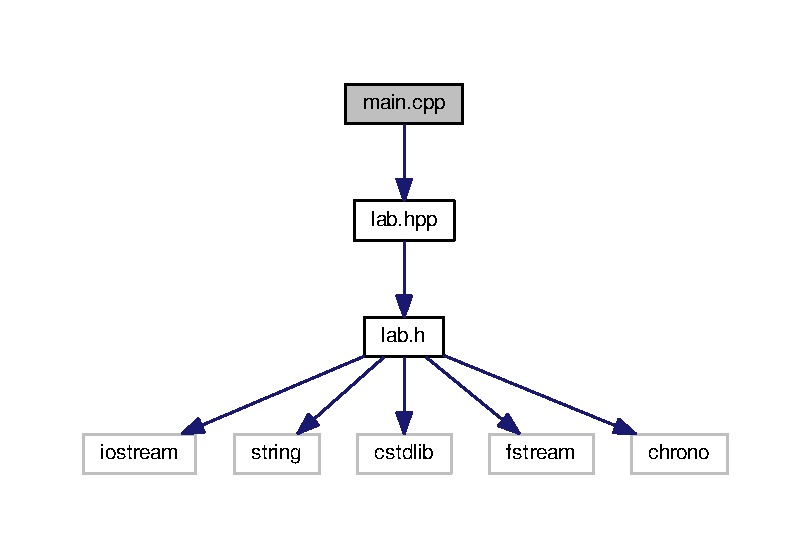
\includegraphics[width=350pt]{main_8cpp__incl}
\end{center}
\end{figure}
\subsubsection*{Functions}
\begin{DoxyCompactItemize}
\item 
int \hyperlink{main_8cpp_ae66f6b31b5ad750f1fe042a706a4e3d4}{main} ()
\end{DoxyCompactItemize}
\subsubsection*{Variables}
\begin{DoxyCompactItemize}
\item 
Fl\+\_\+\+Input $\ast$ \hyperlink{main_8cpp_abf805c82a90897837d1c26ef915f1cd6}{pizza}
\item 
Fl\+\_\+\+Output $\ast$ \hyperlink{main_8cpp_a05c7f6e86cca5f4d0ebf44d1f5042c37}{watch}
\item 
Fl\+\_\+\+Text\+\_\+\+Buffer $\ast$ \hyperlink{main_8cpp_aea2b8efadc87a819fe57c311d668e504}{buff}
\item 
Fl\+\_\+\+Text\+\_\+\+Display $\ast$ \hyperlink{main_8cpp_a23f917547a833922fd6bc8797cc04ee1}{order\+Q}
\end{DoxyCompactItemize}


\subsubsection{Function Documentation}
\hypertarget{main_8cpp_ae66f6b31b5ad750f1fe042a706a4e3d4}{\index{main.\+cpp@{main.\+cpp}!main@{main}}
\index{main@{main}!main.\+cpp@{main.\+cpp}}
\paragraph[{main}]{\setlength{\rightskip}{0pt plus 5cm}int main (
\begin{DoxyParamCaption}
{}
\end{DoxyParamCaption}
)}}\label{main_8cpp_ae66f6b31b5ad750f1fe042a706a4e3d4}

\begin{DoxyCode}
10 \{
11     Fl\_Cairo\_Window cw(400,300); \textcolor{comment}{// width & height of window}
12     cw.label(\textcolor{stringliteral}{"Pizza Deliveries Extravaganja"}); \textcolor{comment}{// title of your cairo window}
13     \textcolor{comment}{//cw.color(FL\_GREEN);}
14     
15     \hyperlink{main_8cpp_abf805c82a90897837d1c26ef915f1cd6}{pizza} = \textcolor{keyword}{new} Fl\_Input(190, 20, 100, 20, \textcolor{stringliteral}{"pizza:"});
16     \hyperlink{main_8cpp_abf805c82a90897837d1c26ef915f1cd6}{pizza}->labelcolor(FL\_BLUE);
17     
18     \hyperlink{main_8cpp_aea2b8efadc87a819fe57c311d668e504}{buff} = \textcolor{keyword}{new} Fl\_Text\_Buffer();
19     \hyperlink{main_8cpp_a23f917547a833922fd6bc8797cc04ee1}{orderQ} = \textcolor{keyword}{new} Fl\_Text\_Display(100,100,100,100,\textcolor{stringliteral}{"Order Q"});
20     \hyperlink{main_8cpp_a23f917547a833922fd6bc8797cc04ee1}{orderQ}->buffer(\hyperlink{main_8cpp_aea2b8efadc87a819fe57c311d668e504}{buff});
21     
22     \hyperlink{main_8cpp_a05c7f6e86cca5f4d0ebf44d1f5042c37}{watch} = \textcolor{keyword}{new} Fl\_Output(70,20,50,20,\textcolor{stringliteral}{"seconds:"});
23     
24     Fl\_Button b(330, 60, 50, 20, \textcolor{stringliteral}{"Order:"});
25     b.callback((Fl\_Callback*)\hyperlink{lab_8h_a547f84331a8c529348e1130ca169c69c}{order\_cb});
26     
27     cw.show();
28     Fl::add\_timeout(1,\hyperlink{lab_8h_a13ed8751dfa95731ad8930762493b16b}{timer});
29     \textcolor{keywordflow}{return} Fl::run();
30 \}
\end{DoxyCode}


\subsubsection{Variable Documentation}
\hypertarget{main_8cpp_aea2b8efadc87a819fe57c311d668e504}{\index{main.\+cpp@{main.\+cpp}!buff@{buff}}
\index{buff@{buff}!main.\+cpp@{main.\+cpp}}
\paragraph[{buff}]{\setlength{\rightskip}{0pt plus 5cm}Fl\+\_\+\+Text\+\_\+\+Buffer$\ast$ buff}}\label{main_8cpp_aea2b8efadc87a819fe57c311d668e504}
\hypertarget{main_8cpp_a23f917547a833922fd6bc8797cc04ee1}{\index{main.\+cpp@{main.\+cpp}!order\+Q@{order\+Q}}
\index{order\+Q@{order\+Q}!main.\+cpp@{main.\+cpp}}
\paragraph[{order\+Q}]{\setlength{\rightskip}{0pt plus 5cm}Fl\+\_\+\+Text\+\_\+\+Display$\ast$ order\+Q}}\label{main_8cpp_a23f917547a833922fd6bc8797cc04ee1}
\hypertarget{main_8cpp_abf805c82a90897837d1c26ef915f1cd6}{\index{main.\+cpp@{main.\+cpp}!pizza@{pizza}}
\index{pizza@{pizza}!main.\+cpp@{main.\+cpp}}
\paragraph[{pizza}]{\setlength{\rightskip}{0pt plus 5cm}Fl\+\_\+\+Input$\ast$ pizza}}\label{main_8cpp_abf805c82a90897837d1c26ef915f1cd6}
\hypertarget{main_8cpp_a05c7f6e86cca5f4d0ebf44d1f5042c37}{\index{main.\+cpp@{main.\+cpp}!watch@{watch}}
\index{watch@{watch}!main.\+cpp@{main.\+cpp}}
\paragraph[{watch}]{\setlength{\rightskip}{0pt plus 5cm}Fl\+\_\+\+Output$\ast$ watch}}\label{main_8cpp_a05c7f6e86cca5f4d0ebf44d1f5042c37}

\hypertarget{Overload_8cpp}{\subsection{Overload.\+cpp File Reference}
\label{Overload_8cpp}\index{Overload.\+cpp@{Overload.\+cpp}}
}
{\ttfamily \#include \char`\"{}lab.\+h\char`\"{}}\\*
Include dependency graph for Overload.\+cpp\+:
\nopagebreak
\begin{figure}[H]
\begin{center}
\leavevmode
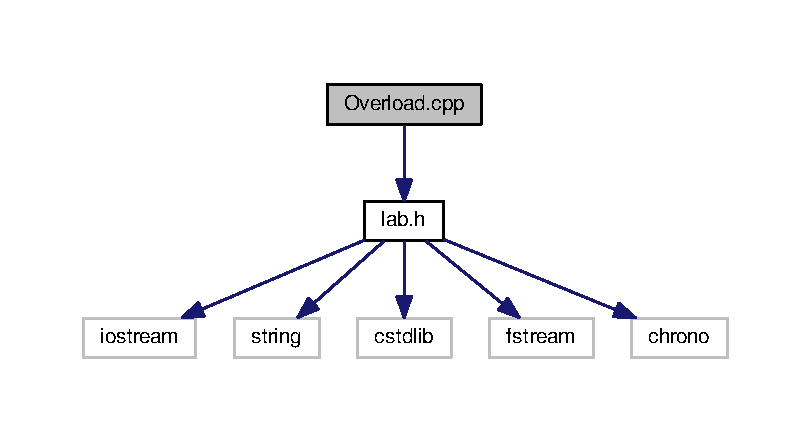
\includegraphics[width=350pt]{Overload_8cpp__incl}
\end{center}
\end{figure}
\subsubsection*{Functions}
\begin{DoxyCompactItemize}
\item 
bool \hyperlink{Overload_8cpp_a93458516135b93160c12abb810a55a99}{operator$<$} (\hyperlink{structAQIData}{A\+Q\+I\+Data} \&lhs, \hyperlink{structAQIData}{A\+Q\+I\+Data} \&rhs)
\item 
bool \hyperlink{Overload_8cpp_a13fdefc73f3cd431a55216baf26cc200}{operator$>$} (\hyperlink{structAQIData}{A\+Q\+I\+Data} \&lhs, \hyperlink{structAQIData}{A\+Q\+I\+Data} \&rhs)
\item 
bool \hyperlink{Overload_8cpp_a2f4ff8cbda09ef68585badaf2bb486f5}{operator$>$=} (\hyperlink{structAQIData}{A\+Q\+I\+Data} \&lhs, \hyperlink{structAQIData}{A\+Q\+I\+Data} \&rhs)
\item 
bool \hyperlink{Overload_8cpp_aef88eef36e8415fda7d0720424b5cf6d}{operator$<$=} (\hyperlink{structAQIData}{A\+Q\+I\+Data} \&lhs, \hyperlink{structAQIData}{A\+Q\+I\+Data} \&rhs)
\end{DoxyCompactItemize}


\subsubsection{Function Documentation}
\hypertarget{Overload_8cpp_a93458516135b93160c12abb810a55a99}{\index{Overload.\+cpp@{Overload.\+cpp}!operator$<$@{operator$<$}}
\index{operator$<$@{operator$<$}!Overload.\+cpp@{Overload.\+cpp}}
\paragraph[{operator$<$}]{\setlength{\rightskip}{0pt plus 5cm}bool operator$<$ (
\begin{DoxyParamCaption}
\item[{{\bf A\+Q\+I\+Data} \&}]{lhs, }
\item[{{\bf A\+Q\+I\+Data} \&}]{rhs}
\end{DoxyParamCaption}
)}}\label{Overload_8cpp_a93458516135b93160c12abb810a55a99}

\begin{DoxyCode}
3 \{
4     \textcolor{keywordflow}{return} (lhs.\hyperlink{structAQIData_a5077140b5e97ceba8b82a776647fb667}{AQI} < rhs.\hyperlink{structAQIData_a5077140b5e97ceba8b82a776647fb667}{AQI});
5 \}
\end{DoxyCode}
\hypertarget{Overload_8cpp_aef88eef36e8415fda7d0720424b5cf6d}{\index{Overload.\+cpp@{Overload.\+cpp}!operator$<$=@{operator$<$=}}
\index{operator$<$=@{operator$<$=}!Overload.\+cpp@{Overload.\+cpp}}
\paragraph[{operator$<$=}]{\setlength{\rightskip}{0pt plus 5cm}bool operator$<$= (
\begin{DoxyParamCaption}
\item[{{\bf A\+Q\+I\+Data} \&}]{lhs, }
\item[{{\bf A\+Q\+I\+Data} \&}]{rhs}
\end{DoxyParamCaption}
)}}\label{Overload_8cpp_aef88eef36e8415fda7d0720424b5cf6d}

\begin{DoxyCode}
17 \{
18     \textcolor{keywordflow}{return} (rhs.\hyperlink{structAQIData_a5077140b5e97ceba8b82a776647fb667}{AQI} <= rhs.\hyperlink{structAQIData_a5077140b5e97ceba8b82a776647fb667}{AQI});
19 \}
\end{DoxyCode}
\hypertarget{Overload_8cpp_a13fdefc73f3cd431a55216baf26cc200}{\index{Overload.\+cpp@{Overload.\+cpp}!operator$>$@{operator$>$}}
\index{operator$>$@{operator$>$}!Overload.\+cpp@{Overload.\+cpp}}
\paragraph[{operator$>$}]{\setlength{\rightskip}{0pt plus 5cm}bool operator$>$ (
\begin{DoxyParamCaption}
\item[{{\bf A\+Q\+I\+Data} \&}]{lhs, }
\item[{{\bf A\+Q\+I\+Data} \&}]{rhs}
\end{DoxyParamCaption}
)}}\label{Overload_8cpp_a13fdefc73f3cd431a55216baf26cc200}

\begin{DoxyCode}
7 \{
8     \textcolor{keywordflow}{return} (lhs.\hyperlink{structAQIData_a5077140b5e97ceba8b82a776647fb667}{AQI} > rhs.\hyperlink{structAQIData_a5077140b5e97ceba8b82a776647fb667}{AQI});
9 \}
\end{DoxyCode}
\hypertarget{Overload_8cpp_a2f4ff8cbda09ef68585badaf2bb486f5}{\index{Overload.\+cpp@{Overload.\+cpp}!operator$>$=@{operator$>$=}}
\index{operator$>$=@{operator$>$=}!Overload.\+cpp@{Overload.\+cpp}}
\paragraph[{operator$>$=}]{\setlength{\rightskip}{0pt plus 5cm}bool operator$>$= (
\begin{DoxyParamCaption}
\item[{{\bf A\+Q\+I\+Data} \&}]{lhs, }
\item[{{\bf A\+Q\+I\+Data} \&}]{rhs}
\end{DoxyParamCaption}
)}}\label{Overload_8cpp_a2f4ff8cbda09ef68585badaf2bb486f5}

\begin{DoxyCode}
12 \{
13     \textcolor{keywordflow}{return} (lhs.\hyperlink{structAQIData_a5077140b5e97ceba8b82a776647fb667}{AQI} >= rhs.\hyperlink{structAQIData_a5077140b5e97ceba8b82a776647fb667}{AQI});
14 \}
\end{DoxyCode}

\hypertarget{readData_8cpp}{\subsection{read\+Data.\+cpp File Reference}
\label{readData_8cpp}\index{read\+Data.\+cpp@{read\+Data.\+cpp}}
}
{\ttfamily \#include \char`\"{}lab.\+h\char`\"{}}\\*
Include dependency graph for read\+Data.\+cpp\+:\nopagebreak
\begin{figure}[H]
\begin{center}
\leavevmode
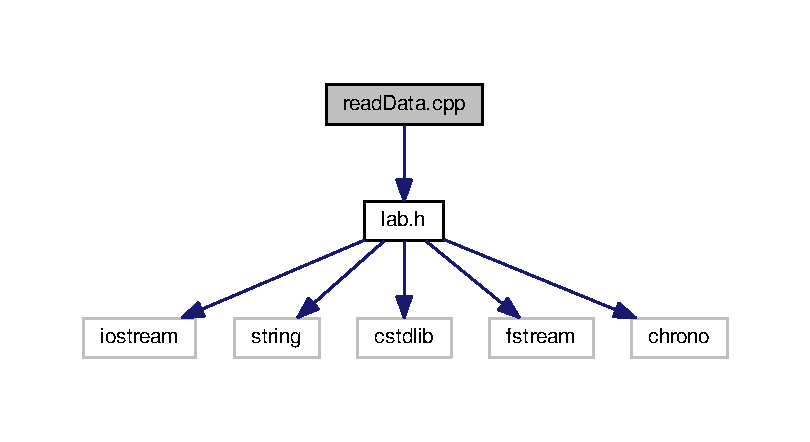
\includegraphics[width=350pt]{readData_8cpp__incl}
\end{center}
\end{figure}
\subsubsection*{Functions}
\begin{DoxyCompactItemize}
\item 
void \hyperlink{readData_8cpp_a3700d6a6f7a91d84cde0120413f3bf38}{read\+Data} (std\+::string f, \hyperlink{structAQIData}{A\+Q\+I\+Data} aqi\mbox{[}$\,$\mbox{]}, int n)
\end{DoxyCompactItemize}


\subsubsection{Function Documentation}
\hypertarget{readData_8cpp_a3700d6a6f7a91d84cde0120413f3bf38}{\index{read\+Data.\+cpp@{read\+Data.\+cpp}!read\+Data@{read\+Data}}
\index{read\+Data@{read\+Data}!read\+Data.\+cpp@{read\+Data.\+cpp}}
\paragraph[{read\+Data}]{\setlength{\rightskip}{0pt plus 5cm}void read\+Data (
\begin{DoxyParamCaption}
\item[{std\+::string}]{f, }
\item[{{\bf A\+Q\+I\+Data}}]{aqi\mbox{[}$\,$\mbox{]}, }
\item[{int}]{n}
\end{DoxyParamCaption}
)}}\label{readData_8cpp_a3700d6a6f7a91d84cde0120413f3bf38}

\begin{DoxyCode}
4 \{
5 
6     std::ifstream ifs(f.c\_str());
7     std::string s; \textcolor{keywordtype}{char} comma;
8     \textcolor{keywordflow}{for}(\textcolor{keywordtype}{int} i = 0; i < n; i++)
9     \{
10         getline(ifs,s,\textcolor{charliteral}{','});\textcolor{comment}{//reads state}
11         getline(ifs,aqi[i].county,\textcolor{charliteral}{','});\textcolor{comment}{//reads county}
12         getline(ifs,s,\textcolor{charliteral}{','});\textcolor{comment}{//ignores county and reads year}
13         getline(ifs,s,\textcolor{charliteral}{','});
14         getline(ifs,s,\textcolor{charliteral}{','});
15         getline(ifs,aqi[i].AQI,\textcolor{charliteral}{','});\textcolor{comment}{//ignore year and readsDays}
16         
17         \textcolor{comment}{//ifs >> aqi[i].AQI >> comma;}
18         getline(ifs,s);
19     \}
20     \textcolor{comment}{//aqi[0].county = s;}
21     ifs.close();
22     
23 
24 \}
\end{DoxyCode}

%--- End generated contents ---

% Index
\newpage
\phantomsection
\addcontentsline{toc}{section}{Index}
\printindex

\end{document}
